\documentclass[a4paper,fontsize=12bp]{extreport}
\usepackage[T2A]{fontenc}
\usepackage[utf8]{inputenc}
\usepackage[english,russian]{babel}
\usepackage[top = 2cm, bottom = 2 cm]{geometry}
\usepackage{cmap}
\usepackage{graphicx}
\usepackage{listings}
\usepackage{color}
\usepackage{amsmath}
\usepackage{pgfplots}
\usepackage{url}
\usepackage{float}
\usepackage{multirow}
\usepackage{indentfirst}
\usepackage[warn]{mathtext} 
\usepackage{wasysym}
\usepackage{scrextend}
\usepackage{titlesec}
\titleformat*{\section}{\LARGE\bfseries}
\titleformat*{\subsection}{\Large\bfseries}
\titleformat*{\subsubsection}{\large\bfseries}
\titleformat*{\paragraph}{\large\bfseries}
\titleformat*{\subparagraph}{\large\bfseries}


\begin{document}

\section*{Задание}

В информационный центр приходят клиенты через интервал времени 10 $\pm$ 2 минуты. Если все три имеющихся оператора заняты, клиенту отказывают в обслуживании. Операторы имеют разную производительность и могут обеспечивать обслуживание среднего запроса пользователя за 20 $\pm$ 5; 40 $\pm$ 10; 40 $\pm$ 20. Клиенты стремятся занять свободного оператора с максимальной производительностью. Полученные запросы сдаются в накопитель. Откуда выбираются на обработку. На первый компьютер запросы от 1 и 2-ого операторов, на второй -- запросы от 3-его. Время обработки запросов первым и 2-м компьютером равны соответственно 15 и 30 мин. Промоделировать процесс обработки 300 запросов. Найти вероятность отказа. 
	
\section*{Теоретическая часть}
	
На рисунке \ref{fig:1} представлена структурная схема концептуальной модели информационного центра.

\begin{figure}[H]
    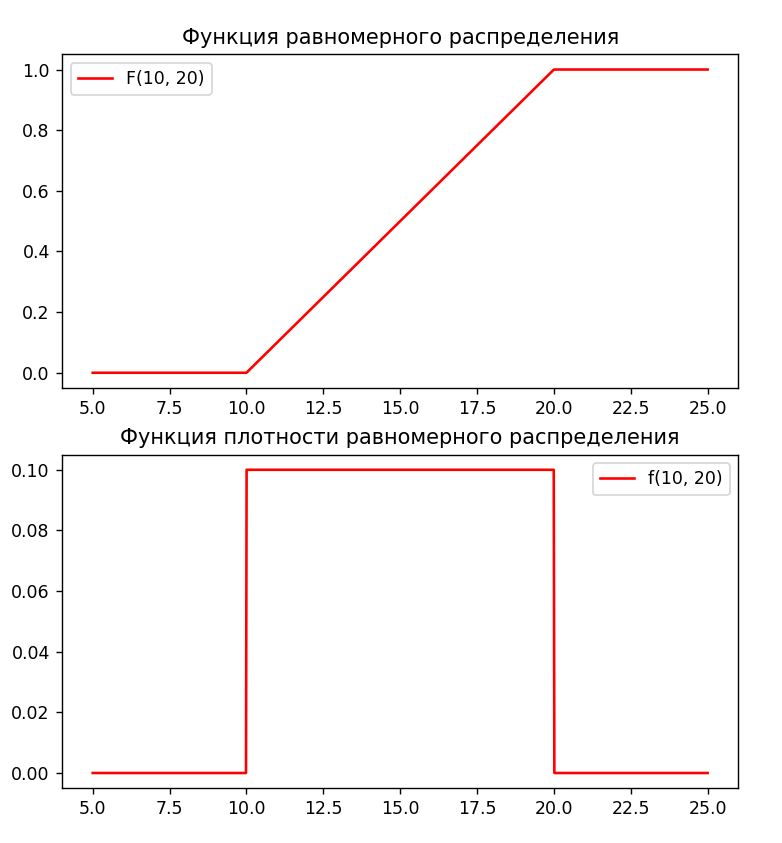
\includegraphics[scale=0.75]{1}
    \caption{Структурная схема}
    \label{fig:1}
\end{figure}

На рисунке \ref{fig:2} представлена концептуальная модель в терминах СМО.
\begin{figure}[H]
    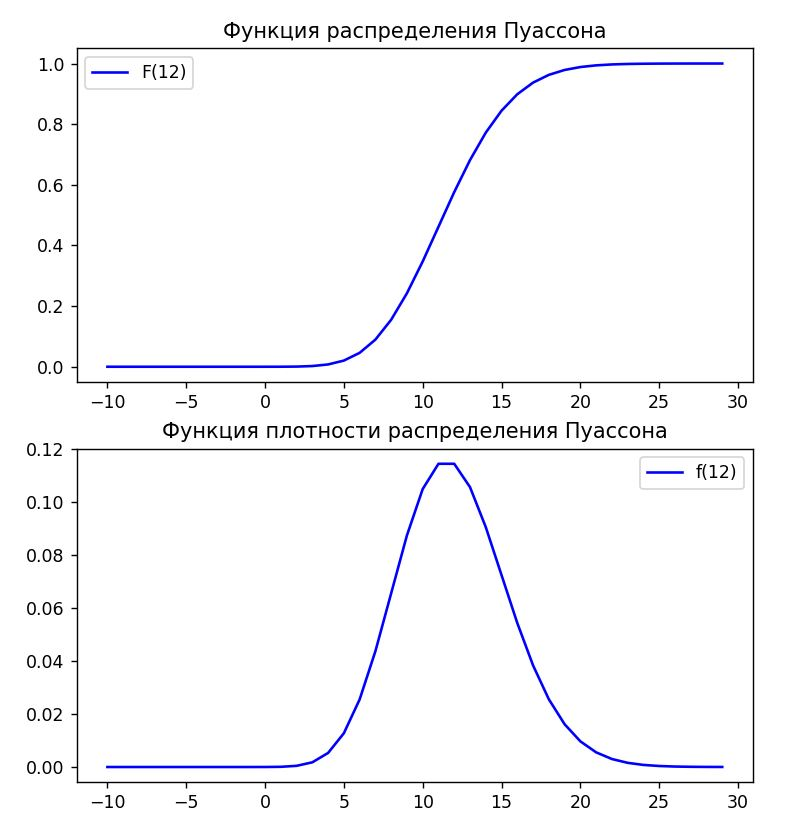
\includegraphics[scale=0.45]{2}
    \caption{Система массового обслуживания}
    \label{fig:2}
\end{figure}

В процессе взаимодействия клиентов с информационным центром возможно:
 \begin{enumerate}
\item Режим нормального обслуживания, т.е. клиент выбирает одного из свободных операторов, отдавая предпочтение тому у которого меньше номер.

\item Режим отказа в обслуживании клиента, когда все операторы заняты
 \end{enumerate}
 
При реализации данной работы используется событийный принцип: состояния отдельных устройств изменяются в дискретные моменты времени, совпадающие с моментами времени поступления сообщений в систему, времени поступления окончания задачи, времени поступления аварийных сигналов и т.д.\\
 
Вероятность отказа находится по следующей формуле:

$$P_\text{отк} = \frac{C_\text{отк}}{C_\text{отк}+C_\text{обсл}}$$

\section*{Листинг}

На рисунке \ref{fig:l} представлен листинг программы.
\begin{figure}[H]
    \includegraphics[scale=0.65]{list.png}
    \caption{Листинг}
    \label{fig:l}
\end{figure}

\newpage
\section*{Результаты работы}

Ниже представлены результаты работы программы.

\begin{figure}[H]
    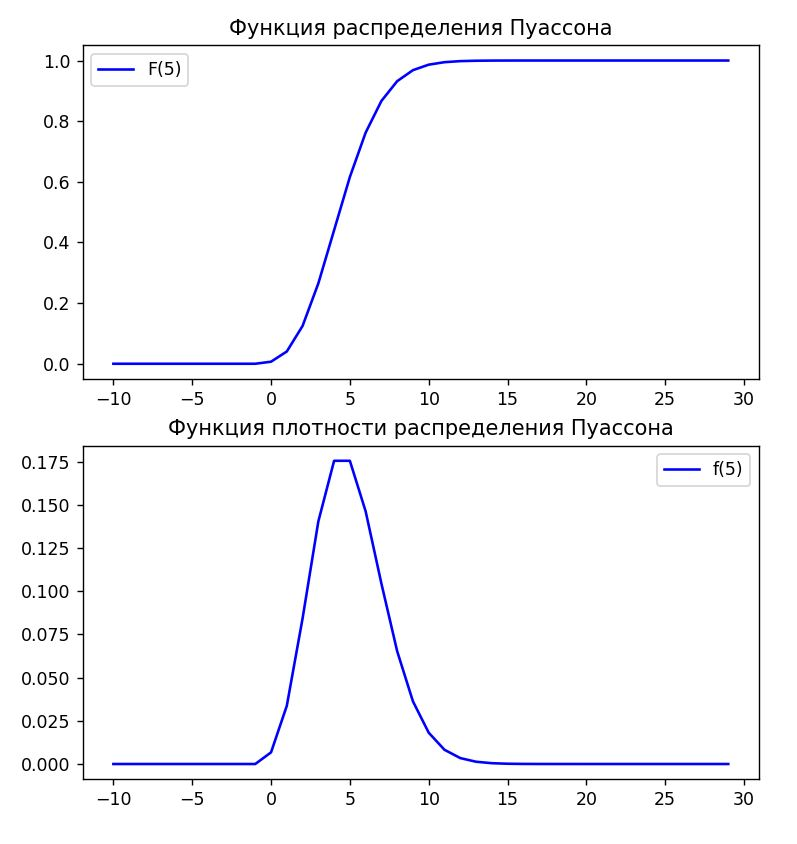
\includegraphics[scale=0.65]{3.png}
    \label{fig:3}
\end{figure}

\begin{figure}[H]
    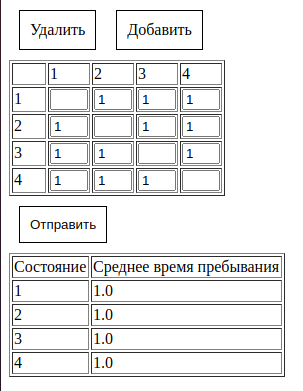
\includegraphics[scale=0.65]{4.png}
    \label{fig:4}
\end{figure}

\begin{figure}[H]
    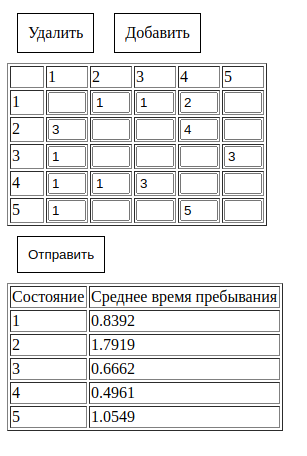
\includegraphics[scale=0.65]{5.png}
    \label{fig:5}
\end{figure}


\section*{Вывод}
В ходе выполнения лабораторной работы был смоделирован информационный центр, найдено количество отказов в обработке, а также вероятность отказа. Вероятность отказа равна 23\%.
\end{document}